% sections/hybrid.tex
\section{Hybrid Perspectives and Future Memory Hierarchies}

Hybrid memory hierarchies aim to combine the high capacity and speed of DRAM with the non-volatility and instant resume capability of FeRAM (including FeFET variants). 
By placing FeRAM near the memory controller or integrated as chiplets alongside DRAM, systems can reduce refresh energy, enable instant-on functionality, and support fast checkpointing and recovery.

% --- Fig.5: Hybrid hierarchy schematic (with SystemDK) ---
\begin{figure}[!t]
  \centering
  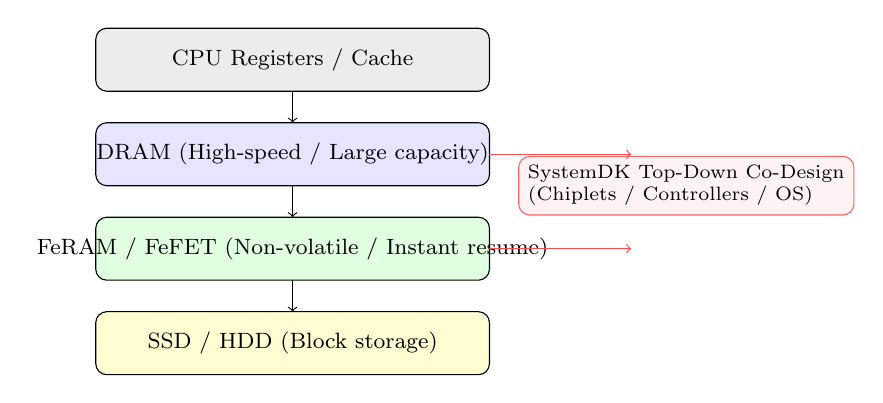
\begin{tikzpicture}[font=\footnotesize]

    % CPU/Cache
    \draw[fill=gray!15, rounded corners] (-2.5,3.0) rectangle (2.5,3.8);
    \node at (0,3.4) {CPU Registers / Cache};

    % DRAM
    \draw[fill=blue!10, rounded corners] (-2.5,1.8) rectangle (2.5,2.6);
    \node at (0,2.2) {DRAM (High-speed / Large capacity)};

    % FeRAM
    \draw[fill=green!12, rounded corners] (-2.5,0.6) rectangle (2.5,1.4);
    \node at (0,1.0) {FeRAM / FeFET (Non-volatile / Instant resume)};

    % SSD/HDD
    \draw[fill=yellow!18, rounded corners] (-2.5,-0.6) rectangle (2.5,0.2);
    \node at (0,-0.2) {SSD / HDD (Block storage)};

    % Arrows
    \draw[->] (0,3.0) -- (0,2.6);
    \draw[->] (0,1.8) -- (0,1.4);
    \draw[->] (0,0.6) -- (0,0.2);

    % SystemDK annotation (right side)
    \node[align=left, draw=red!60, rounded corners, fill=red!5, font=\scriptsize] 
      at (5.0,1.8) {SystemDK Top-Down Co-Design\\(Chiplets / Controllers / OS)};
    \draw[->, red!70] (2.5,2.2) -- (4.3,2.2);
    \draw[->, red!70] (2.5,1.0) -- (4.3,1.0);

  \end{tikzpicture}
  \caption{Hybrid memory hierarchy integrating DRAM (high-speed capacity) and FeRAM (persistent supplement). 
  SystemDK enables top-down co-design across chiplets, controllers, and OS.}
  \label{fig:hybrid_hierarchy}
\end{figure}

\subsection*{Benefits}
\begin{itemize}
  \item \textbf{Reduced refresh overhead:} FeRAM can hold cold pages or metadata, cutting DRAM refresh traffic and standby power.
  \item \textbf{Fast persistence:} OS and application state can be checkpointed to FeRAM with microsecond-scale latency.
  \item \textbf{Data resilience:} FeRAM provides crash consistency for critical metadata and write-back buffers.
\end{itemize}

\subsection*{Constraints and trade-offs}
\begin{itemize}
  \item \textbf{Endurance and variability:} FeRAM endurance ($10^{12}$--$10^{13}$ cycles) is high but below effective DRAM activity levels.
  \item \textbf{Write energy and latency:} Higher than DRAM; cold or read-mostly data should be placed in FeRAM.
  \item \textbf{Integration cost:} Ferroelectric layers or FeFET adoption adds process and reliability risks (e.g., high-field stress).
\end{itemize}

\subsection*{System-level directions}
\begin{itemize}
  \item \textbf{Tiering policies:} Classify pages/objects by write intensity and retention needs, migrating cold or persistent data to FeRAM.
  \item \textbf{Refresh co-optimization:} Dynamically shrink DRAM refresh for regions shadowed or backed by FeRAM.
  \item \textbf{Controller/OS support:} Metadata for wear tracking, retention-aware placement, and error telemetry.
  \item \textbf{SystemDK co-design:} Enable holistic optimization from chiplets to OS in one design flow.
\end{itemize}
